%%% note.tex ---

%% Author: Yi Cao
%% Version: $Id: note.tex,v 0.0 2017/01/22 06:08:01 ycao

%% revision: note.tex,v 0.0 2017/01/22 06:08:01 ycao

%%%---------------------------------------------------------------------

\documentclass[11pt]{article}
\usepackage[letterpaper, portrait, top=1in, bottom=1in, left=1in, right=1in]{geometry}
\usepackage{fancyhdr}
\usepackage{lastpage}
\usepackage{graphicx}
\pagestyle{fancy}
\lhead{\textbf{Young Type Ia Supernovae}}
\rhead{\textbf{Yi Cao}}
\cfoot{\thepage/\pageref{LastPage}}
\usepackage{multicol}
\usepackage[font=small, labelfont=bf]{caption}
\usepackage{wrapfig}
\usepackage[shortlabels]{enumitem}
\usepackage{amssymb}
\usepackage{amsmath}
\setlength{\multicolsep}{2.0pt plus 2.0pt minus 1.5pt}
\usepackage{url}



\begin{document}

%%%%##########################################################################

\begin{center}
  \textbf{\Large Emission From Young Type Ia Supernovae}\\
  Last Update: \today
\end{center}

\section{Introduction}
\label{sec:introduction}

Observations of Type Ia supernovae (SNe Ia) within a few days of
explosion is a promising avenue to further constrain the progenitor
systems and explosion mechanisms of these SNe. This note summarizes
theoretical and observational results in this field together with my
thoughts towards future developement. The organization of this note is
as follows: Section \ref{sec:introduction} discusses the SN shock
breakout. Section \ref{sec:sn_companion_collision} talks about the
SN-companion collisioin. Section
\ref{sec:diversity_of_radioactively_powered_light_curves} talks about
the diversity of radioactively powered light curves. Section
\ref{sec:sn_csm_interaction} presents possible signatures from SN-CSM
interaction. In addition, some of the thoughts are applicable to Type
Ibc supernovae (SNe Ibc), which is discussed in Section
\ref{sec:thoughts_on_type_ibc_sne}.

\section{SN Shock Breakout}
\label{sec:sn_shock_breakout}

A SN explosion begins with a SN shock breaking out of the surface of
the exploding star. The shock breakout occurs when the opacity in
front of the radiatively-driven SN shock drops to $\sim c/v_{sh}$,
where $c$ is the speed of light and $v_{sh}$ is the speed of the shock
wave.  The shock breakout produces a bright flash in the X-ray on the
light crossing timescale. Thanks to the small size of the progenitor
star (a white dwarf), the timescale for shock breakout in a SN Ia is
subsecond. Therefore, it is not feasible to catch this signal with any
current X-ray instrument except for serendipitous discoveries.

Following the shock breakout, the heated and unbinded envelops in the
exploding star (the ejecta) starts to expand rapidly, giving off
thermal emissions. This adiabatic and free expanding phase has been
approached by multiple theoretical models (e.g., Piro, Chang \&
Weinberg 2010; Rabinak \& Waxman 2011). Despite subtle differences in
assumptions on ejecta profiles and opacity, these models give similar
predictions on the light curve. The successful application of these
models to SN2011fe (Bloom et al. 2012) led to a strong constraint on
the size of its progenitor star ($\lesssim0.02R_\odot$; see Figure
\ref{fig:shock_breakout}). A caveat here is that this result strongly
depends on the assumption on the exact explosion time of the SN. Piro
\& Nakar (2014) argued that SN2011fe may have experienced a dark period of
$\sim$ a day before the rise of its radioactively powered light curve.

\begin{figure}[htb]
  \centering
  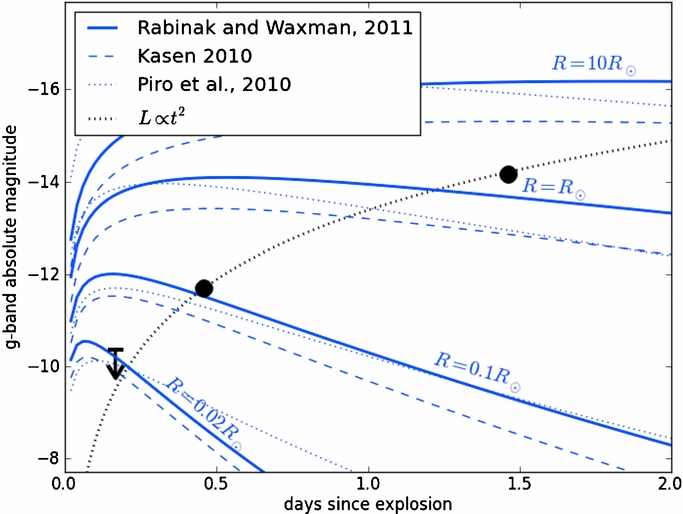
\includegraphics[width=0.9\textwidth]{shock_breakout.jpg}
  \caption{SN-Shock cooling models are compared to early observations
    of SN2011fe. [Figure 2 in Bloom et al. (2012)]}
  \label{fig:shock_breakout}
\end{figure}

According to Figure \ref{fig:shock_breakout}, the shock cooling light
curve peaks at $g\simeq -10.5\,\textrm{mag}$ within $0.1$ day of the
SN explosion.  Hence, this cooling phase can only be caught by an
extremely fast cadence transient survey (something like a two-hour
cadence) of very nearby galaxies. For example, with a detection limit
of $g=21.5\,\textrm{mag}$, this measurements can be undertaken for SNe
in galaxies up to a distance modulus of $\mu=32\,\textrm{mag}$. The
all-sky SN Ia rate within this distance is $0.07$ per year,
unfortunately.


\section{SN-Companion Collision}
\label{sec:sn_companion_collision}

If a SN is born in the single-degenerate channel, its companion may
still be alive at the time of the SN explosion. Thus the inevitable
collision bewteen the SN ejecta and the companion may produce visible
signatures in the early light curve of the SN, which could serve as a
``smoking gun'' for the single-degenerate channel. In contrast, this
SN-companion collision signature is not expected in the
double-degenerate scenario.

On the theory side, Kasen (2010) provided the currently
widely-accepted model that describes the expected signature from the
SN-compaion collision (there are a few other papers debating the
impact of the collision on the color of the SNe at peak). It also
provided analytical equations for convenient comparison to
observations. On the observation side, searching for the SN-companion
collision signatures has been carried out in a few optical surveys
(Hayden et al. 2010; Bianco et al. 2011), but their cadences and
sensitivities were not ideal to catch this signature, so it is not
surprising that these searches ended up with null detection. Brown et
al. (2012a) also looked at archival Swift data of SNe Ia (very few of
them were observed within five days of explosions) and reported
non-detection in any of the observed SNe. Recent fast-cadence optical
surveys, such as (i)PTF and ASAS-SN, have allowed researchers to
rapidly trigger UV follow-up observations for individual nearby events
in order to look for this signature. Brown et al. (2012b) reported
non-detection of this signature in the early observation of
SN2011fe. Cao et al. (2015) reported first detection of a strong and
declining UV emission from a young low-velocity SN Ia iPTF14atg, which
is consistent with expectation of SN-companion collision.  Marion et
al. (2016) reportedly attribute a possible excess in the early
emission of SN2012cg to the SN-companion collision, but this result
was strongly questioned recently (e.g., Shappee et al. 2016 arXiv:
161007601).

Assuming an ejecta mass of $1.4M_\odot$ and an expansion velocity of
$10^9\,\textrm{km}\,\textrm{s}^{-1}$, we use Kasen's model to
calculate the expected light curves of SN-companion collision in
different filters. The angular dependence of the light curves is
approximated by the parameterized equation from Brown et al. (2012a).
If we fix the binary separation at $a=10^{13}\,\textrm{cm}$, the
expected light curves at different viewing angles in the UVOT
\textit{uvm2} (the UVOT \textit{uvm2} bandpass is very similar to the
bandpass of the proposed ULTRASAT), PTF \textit{g}, and PTF \textit{R}
bands are shown in Figures \ref{fig:sn_companion_g_band},
\ref{fig:sn_companion_R_band} and \ref{fig:sn_companion_uvm2_band},
respectively. Figure \ref{fig:sn_companion_range} also shows the
absolute magnitude range of SN-companion collision as a function of
binary separation at one day after explosion.

We conclude from these figures that near-UV is a much more preferred
waveband to detect the SN-companion collision signature than
optical. First, the signature in the near-UV is brighter than that in
the optical by a couple of magnitude. Second, the contrast between the
SN-companion collision signature and the SN photospheric emission is
much greater in the near-UV than in the optical. We may still detect a
clear signal of SN-companion collision in the near-UV even 3 -- 4 days
after the explosion. The downside of the near-UV is much more
sensitive to extinction.

\begin{figure}[htb]
  \centering
  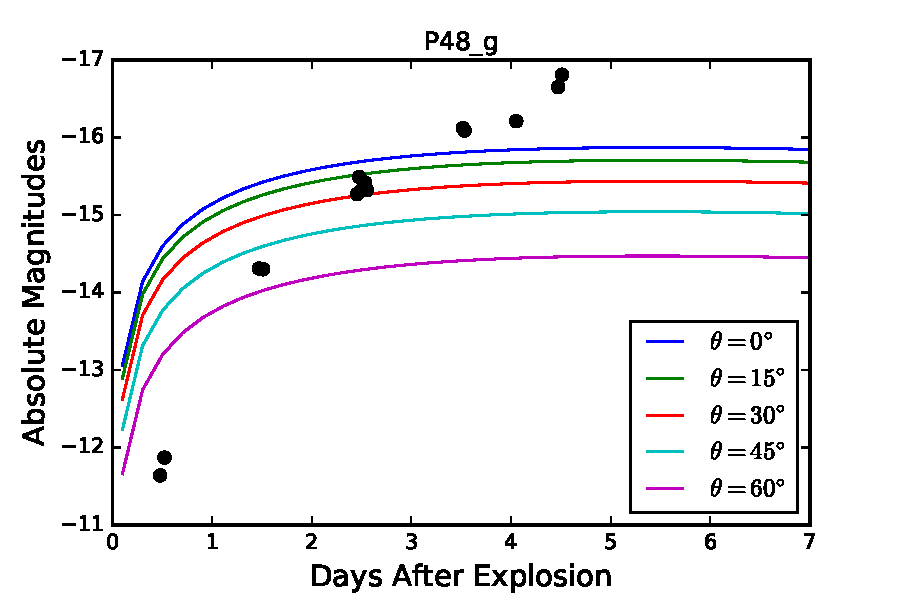
\includegraphics[width=0.9\textwidth]{P48_g.pdf}
  \caption{Theoretical \textit{g}-band light curves of SN-companion
    collision in a binary separating by $10^{13}\,\textrm{cm}$. The
    black circles show the observed light curve of SN2011fe. }
\label{fig:sn_companion_g_band}
\end{figure}

\begin{figure}[htb]
  \centering
  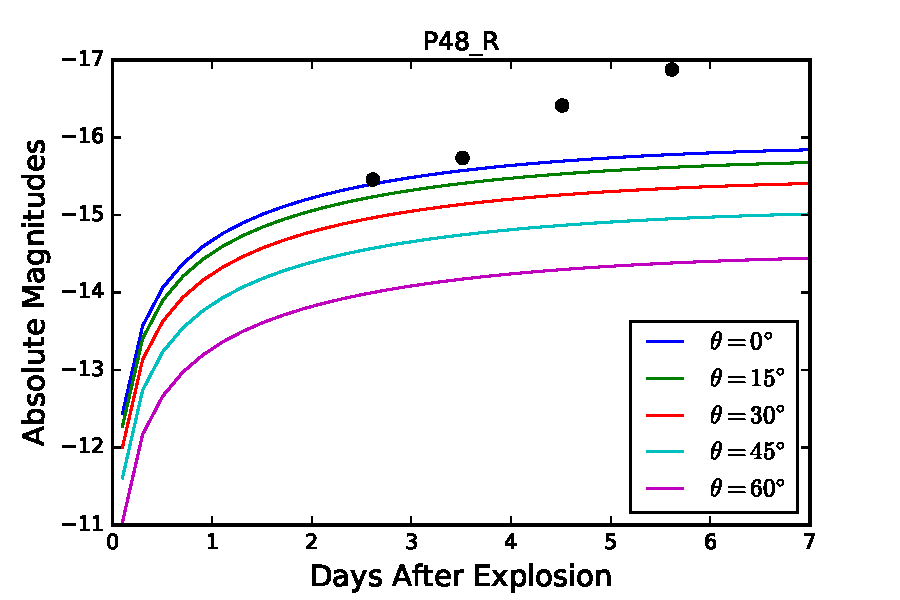
\includegraphics[width=0.9\textwidth]{P48_R.pdf}
  \caption{Same as Figure \ref{fig:sn_companion_g_band}, but in the \textit{R} band.}
  \label{fig:sn_companion_R_band}
\end{figure}

\begin{figure}[htb]
  \centering
  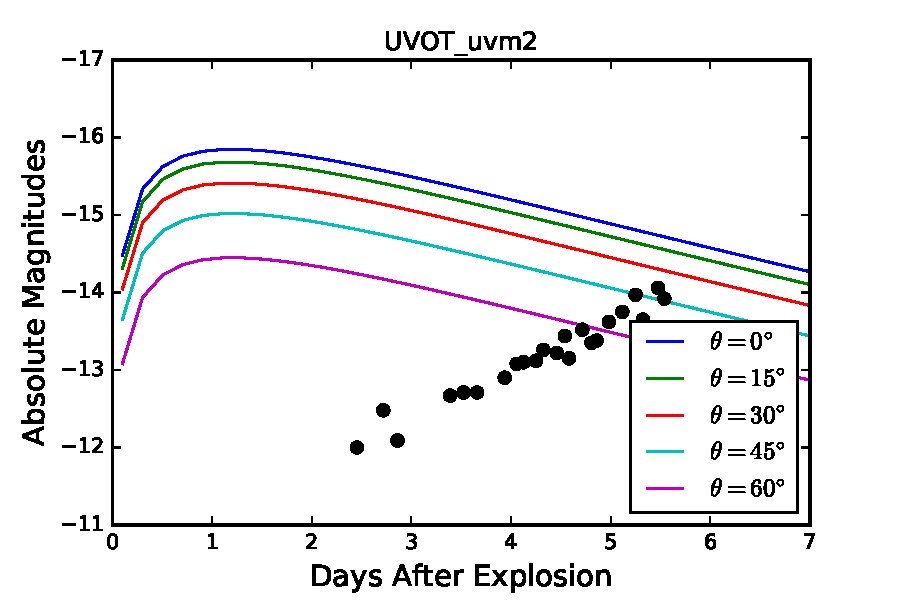
\includegraphics[width=0.9\textwidth]{UVOT_uvm2.pdf}
  \caption{Same as Figure \ref{fig:sn_companion_g_band}, but in the UVOT \textit{uvm2} band.}
  \label{fig:sn_companion_uvm2_band}
\end{figure}

\begin{figure}[htb]
  \centering
  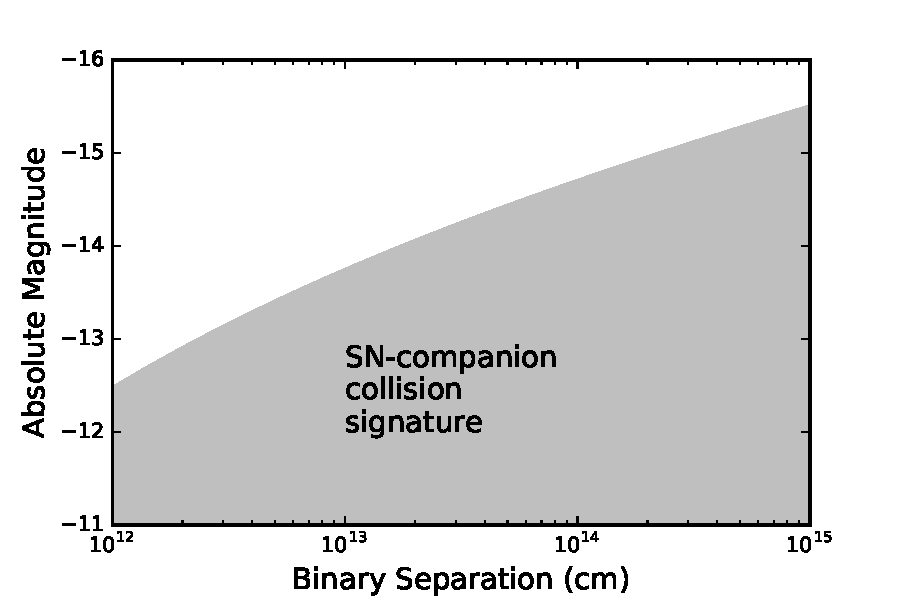
\includegraphics[width=0.9\textwidth]{g_band_a_vs_theta.pdf}
  \caption{The absolute \textit{g}-band magnitude range of
    SN-companion collision (gray region) at one day after explosion as
    a function of the binary separation}
  \label{fig:sn_companion_range}
\end{figure}

\section{Diversity Of Radioactively Powered Light Curves}
\label{sec:diversity_of_radioactively_powered_light_curves}

The radioactively powered light curve does not rise until the energy
of radioactive decay diffuses to the photosphere. Thus a SN may
experience a dark period after the SN shock breakout. For example,
Piro \& Nakar (2014) claimed that SN2011fe had a period of one day,
and consequently the tight constraint on the size of the progenitor
derived in Bloom et al. (2012) does not hold. Constraining the dark
period of a SN Ia not only improves estimates of its rise time and
thus its ejecta and total $^{56}$Ni masses, but also provides further
constraints on the mixing of nucleosynthesis in the SN explosion.

Recently, Piro \& Morozova (2016) presented theoretical early light
curves for both weak and strong mixing in the ejecta. Figure
\ref{fig:deposition} illustrates that the initial rise rate of the
light curve is correlated with the degree of mixing in the ejecta:
strong mixing leads to an early and fast-initial-rise light curve,
while weak mixing leads to a delayed and slow-initial-rise light
curve. Therefore measuring the rise rate in the first day of the light
curve provides a useful tool to estimate the length of the dark
period.

\begin{figure}[htb]
  \centering
  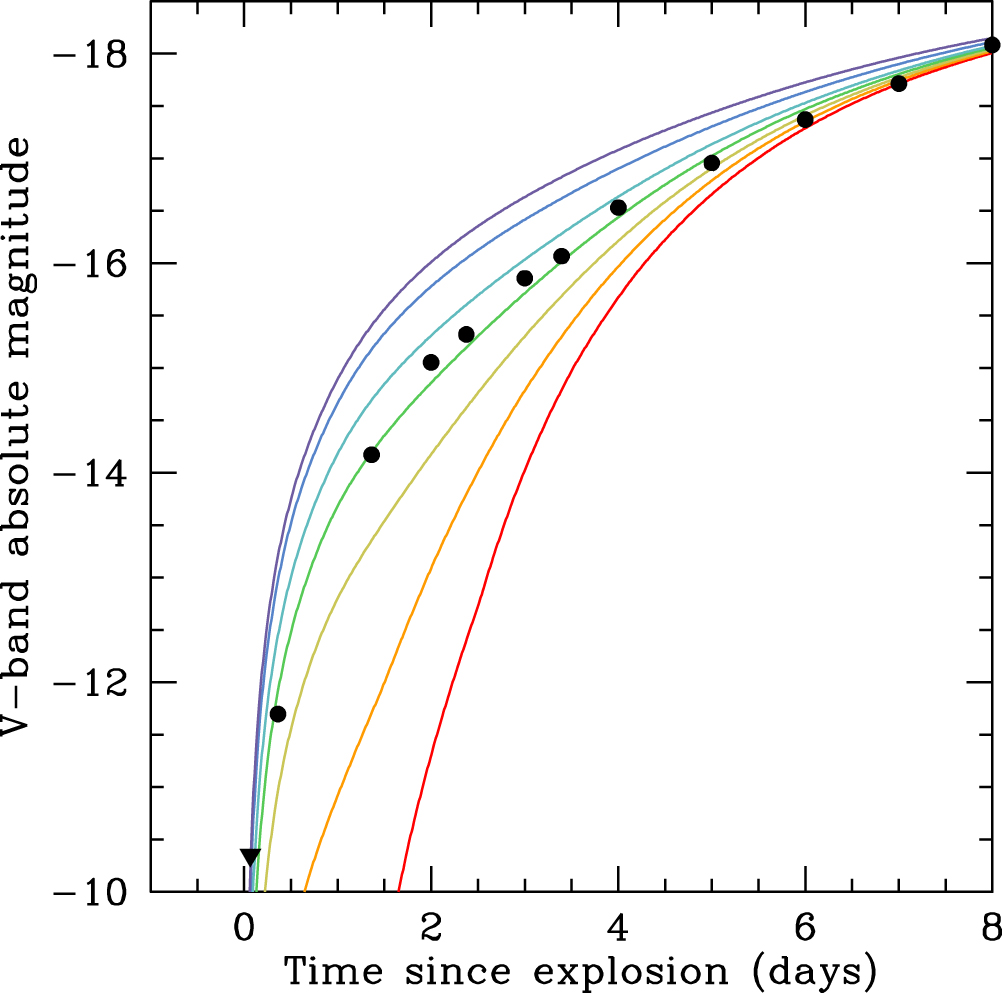
\includegraphics[width=0.9\textwidth]{deposition.jpg}
  \caption{The radioactively powered light curves from the ejecta of
    weak (red) and strong (blue) mixing. The circles and triangle are
    the observed light curve of SN2011fe. [Figure 7 in Piro \&
    Morozova (2016)] }
  \label{fig:deposition}
\end{figure}

I want to emphasize that the diversity of the early light curve
arising from mixing of $^{56}$Ni is distinguishable in observations
from that of the SN-companion collision signature at various viewing
angles. The former emission is generated by the photosphere heated up
continuously by radioactive decay energy, while the latter emission
follows the cooling of the SN-companion collision. Thus these two
scenarios lead to distinct evolution of photospheric temperatures and
can be distinguished by SN color evolution.

\section{SN-CSM Interaction}
\label{sec:sn_csm_interaction}

Most progenitor scenarios of SNe Ia involve some sort of mass transfer
process, which in principle should leave excess material around the
exploding star. This circumstellar material may interact with the SN
ejecta and produce signals on the SN light curve and spectra. For
example, some SNe Ia show varying Na\,I\,D absorption (e.g., Sternberg
et al. 2011). A special subtype of SNe Ia, called SNe Ia-CSM, have
also been identified (e.g., Silverman et al. 2013). Observations of
these SNe at very young age may provide diagnostics to the mass loss
history of the progenitor systems. So far, to my knowledge, none of
these events has very early data.

First, existence of an extended material around the SN progenitor will
produce an extra peak in the very early light curve (Figure
\ref{fig:extended_material}). This peak is due to the cooling of the
material in the circumstellar medium after the SN shock heats it up.
The duration and amplitude of this early peak can be used to estimate
the mass and location of the circumstellar material (Piro \& Morozova
2016).

\begin{figure}[htb]
  \centering
  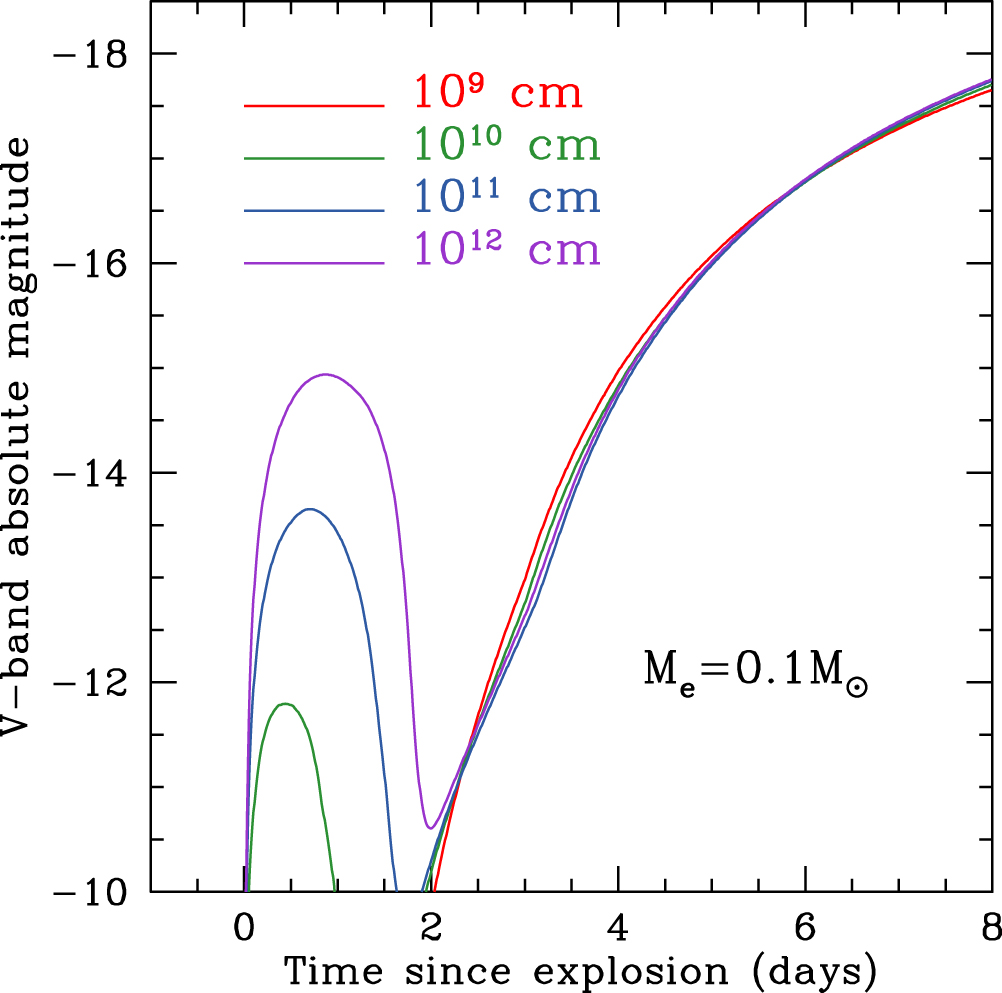
\includegraphics[width=0.9\textwidth]{extended_material.jpg}
  \caption{The early light curve peak produced by an extended material
    of $0.1M_\odot$ at different distances. [Figure 10 in Piro \&
    Morozova (2016)]}
  \label{fig:extended_material}
\end{figure}

Separately, analogous to flash signature in the earliest spectra of
SNe II (Gal-Yam et al. 2014), high energy photons from the SN
explosion may ionize the circumstellar medium. The consequent
recombination emission lines may appear in the earliest spectra of a
SN Ia-CSM. These recombination lines are very useful to probe the
chemical abundance and density profile of the circumstellar medium.


\section{Some Thoughts On Type Ibc SNe}
\label{sec:thoughts_on_type_ibc_sne}

\textbf{ycao: need more references in this section}

The ideas presented in Sections \ref{sec:sn_companion_collision} and
\ref{sec:diversity_of_radioactively_powered_light_curves} may also be
applicable to SNe Ibc, however, with very large uncertainties. Both
observational and theoretical work is warranted to make progresses
here.

Mass loss history plays an important role in the evolution of SN Ibc
progenitors. There are two scenarios: a Wolf-Rayet star strips its
hydrogen and (part of) helium layers through strong stellar winds; a
less massive star removes its outer envelope by close binary
interaction. Observations of the only identified progenitor system of a
Type Ib SN iPTF13bvn (Folatelli et al. 2016; Eldridge \& Maund 2016).

The SN-companion collision signature may also be used to distinguish
these two scenarios. However, the opening angle of the companion star
in the binary system is in general much smaller than that in the
single-degenerate channel of SNe Ia, because the binary progenitors of
SNe Ibc are not necessarily close enough to enable Roche lobe mass
transfer. Therefore, the chance for us to see the SN-companion
collision signature is very low.

If the material stripped from the progenitor star of a SN Ibc stays
close at the time of explosion, we should also expect to see an extra
peak in the light curve, which is generated by the cooling of the
extended material, and recombination lines in the early spectra, which
are produced by the extended material ionized by the high-energy
photons from the SN. In fact, we have seen both signatures in a few
cases in iPTF. For example, Type Ic SN iPTF15dtg showed a
double-peaked light curve (Taddia et al. 2016). Although the exact
type of iPTF14gqr is still in debate (Ca-rich vs Type Ibc), it shows a
double-peaked light curve, with its first peak decaying within three
days of explosion. The spectra taken during its first peak show He\,II
4686, C\,IV 4650 and C\,IV 5806, hallmark lines of flash spectroscopy.

%%%%##########################################################################

\end{document}
